\documentclass[11pt,a4paper,twoside,openright]{report}

% --- pacotes essenciais -------------------------------------------------
\usepackage[utf8]{inputenc}
\usepackage[T1]{fontenc}
\usepackage[portuguese]{babel}
\usepackage{graphicx}
\usepackage{amsmath}
\usepackage{amssymb}
\usepackage{geometry}
\usepackage{acronym}
\usepackage{hyperref}
\usepackage{url}
\usepackage{enumitem}
\usepackage{booktabs}
\usepackage{caption}
\usepackage{indentfirst}
\usepackage{xcolor}

\geometry{a4paper, margin=2.5cm}

\hypersetup{
    colorlinks=true,
    linkcolor=black,
    citecolor=black,
    urlcolor=blue
}

% --- inicio do documento ------------------------------------------------
\begin{document}

% capa
\thispagestyle{empty}
\setcounter{page}{-1}
\begin{center}
\begin{Huge}
\textbf{Universidade da Beira Interior}
\end{Huge}
\end{center}
\begin{center}
\begin{Huge}
Departamento de Informática
\end{Huge}
\end{center}
\vspace{0,07cm}
\begin{figure}[!htb]
\centering

\includegraphics[width=180pt]{ubi-fe-di.png}
\end{figure}
\vspace{0.5cm}
\begin{center}
\begin{Large}
\textbf{Elementos de Inteligência Artificial e Ciência de Dados}
\end{Large}
\end{center}
\vspace{0.3cm}
\begin{center}
\begin{Large}
\emph{Análise de Dados Aplicada ao Acompanhamento Nutricional}
\end{Large}
\end{center}
\vspace{0.5cm}
\begin{center}
\begin{normalsize}
\begin{large}
Elaborado por:
\end{large}
\end{normalsize}
\end{center}
\vspace{0.3cm}
\begin{center}
\begin{large}
\textbf{Leandro Apolo  N: 55459} \\
\textbf{Jorge Altamirano  N: [NÚMERO]} \\
\textbf{Jose Gordon  N: [NÚMERO]}
\end{large}
\end{center}
\vspace{0,5cm}
\begin{center}
\begin{normalsize}
\begin{large}
Docentes:
\end{large}
\end{normalsize}
\end{center}
\vspace{0.2cm}
\begin{center}
\begin{large}
\textbf{Professor João C. Neves} \\
\textbf{Professor Tiago Filipe Dias dos Santos Roxo}
\end{large}
\end{center}
\vspace{0.5cm}
\begin{center}
\begin{normalsize}
\today
\end{normalsize}
\end{center}


% paginas iniciais sem numeracao de capitulo
\pagenumbering{roman}

\chapter*{Agradecimentos}
\label{chap:ack}

A conclusão deste trabalho não seria possível sem o apoio de várias pessoas a quem o grupo deixa o seu sincero agradecimento.

Agradecemos aos docentes da unidade curricular de \ac{EIACD} pela orientação, pelo enunciado bem estruturado e pela disponibilidade demonstrada ao longo do semestre.

Agradecemos também aos colegas pela troca de ideias durante o desenvolvimento, e à \ac{UBI} pelas condições proporcionadas para a realização deste projeto.

\newpage

\tableofcontents
\newpage

\listoffigures
\newpage

\listoftables
\newpage

\chapter*{Acrónimos}
\label{chap:acro}

\begin{acronym}[CFIUTE]
  \acro{EIACD}{Elementos de Inteligência Artificial e Ciência de Dados}
  \acro{CSV}{\emph{Comma-Separated Values}}
  \acro{IMC}{Índice de Massa Corporal}
  \acro{UBI}{Universidade da Beira Interior}
\end{acronym}

\newpage

% corpo do documento
\pagenumbering{arabic}

\chapter{Introdução}
\label{chap:intro}

\section{Enquadramento}
A prevalência de doenças crónicas associadas a hábitos alimentares inadequados, como a obesidade, a diabetes tipo 2 e as doenças cardiovasculares, tem aumentado a atenção dada à nutrição como fator de saúde. Neste contexto, o acompanhamento nutricional personalizado tornou-se uma ferramenta relevante na promoção de estilos de vida mais saudáveis e na melhoria dos indicadores clínicos dos pacientes.

A eficácia de uma dieta não depende apenas do plano alimentar em si. Depende também de fatores biológicos do paciente, do seu comportamento e nível de adesão, e até do perfil do profissional que faz o acompanhamento. Esta combinação de fatores torna difícil prever, à partida, que planos têm maior probabilidade de sucesso para um determinado perfil de paciente.

\section{Motivação}
O interesse deste problema está em perceber se os dados recolhidos durante o acompanhamento nutricional contêm informação suficiente para antecipar resultados. Se for possível estimar com alguma fiabilidade quanto peso um paciente vai perder, ou se uma dieta tem boa probabilidade de sucesso, então essa informação pode apoiar decisões clínicas antes de a dieta começar.

O grupo abordou o problema através de um conjunto de dados que reúne informação sobre pacientes, planos dietéticos, nutricionistas responsáveis e resultados das dietas ao fim de seis meses. O objetivo foi explorar e caracterizar esses dados, identificar padrões associados ao sucesso ou insucesso das dietas, e construir modelos capazes de fazer previsões úteis.

\section{Objetivos}
O trabalho consistiu na construção de um conjunto de \textit{scripts} em Python que executam, de forma encadeada, todas as etapas de um processo de análise de dados. As etapas vão desde a integração dos quatro ficheiros \ac{CSV} fornecidos até à aplicação de modelos de previsão e à discussão crítica dos resultados obtidos.

Em concreto, os objetivos foram integrar os dados num único conjunto, limpar e transformar esse conjunto, realizar uma análise exploratória detalhada, identificar grupos de pacientes através de \textit{clustering}, treinar modelos supervisionados para prever a perda de peso, e por fim comparar e discutir o desempenho desses modelos.

\section{Organização do Documento}
O documento está organizado em seis capítulos. Depois desta introdução, o segundo capítulo descreve a integração dos dados e a estrutura do conjunto unificado. O terceiro apresenta a limpeza e o processamento aplicados. O quarto descreve a análise exploratória e os padrões diretos encontrados. O quinto trata da identificação de padrões por \textit{clustering} e da aplicação dos modelos de previsão. O último capítulo apresenta a discussão crítica dos resultados e as conclusões do trabalho.

\chapter{Integração de Dados}
\label{chap:integracao}

\section{Os Quatro Ficheiros de Origem}
Os dados foram fornecidos em quatro ficheiros \ac{CSV} distintos, cada um correspondente a uma parte do problema. O ficheiro \texttt{patients.csv} contém os registos dos pacientes, com 1000 linhas e atributos como sexo, idade, altura, peso inicial, \ac{IMC}, hábito tabágico, horas de sono e um indicador de motivação. O ficheiro \texttt{nutritionists.csv} descreve os 20 nutricionistas, com a sua abordagem de acompanhamento, anos de experiência e especialidade. O ficheiro \texttt{diets.csv} caracteriza os 10 planos alimentares, indicando o tipo de dieta e a sua composição em macronutrientes. Por fim, o ficheiro \texttt{outcomes.csv} regista 2523 programas de dieta, cada um ligando um paciente, um nutricionista e uma dieta a um resultado medido ao fim de seis meses.

A relação entre os ficheiros faz-se através de identificadores. Cada programa em \texttt{outcomes.csv} refere um \texttt{patient\_id}, um \texttt{nutritionist\_id} e um \texttt{diet\_id}, que funcionam como chaves para os outros três ficheiros.

\section{Estratégia de Junção}
A integração foi implementada no \textit{script} \texttt{data\_integration.py}, recorrendo à biblioteca \textit{pandas}~\cite{pandas}. O grupo optou por usar o ficheiro \texttt{outcomes.csv} como tabela central, uma vez que é o que tem mais linhas e o que representa a unidade de análise do problema, ou seja, um programa de dieta com o seu resultado.

A partir dessa tabela central foram feitas três junções do tipo \textit{left join}. A primeira liga cada programa aos dados do respetivo paciente pela coluna \texttt{patient\_id}. A segunda junta as características da dieta pela coluna \texttt{diet\_id}. A terceira acrescenta a informação do nutricionista pela coluna \texttt{nutritionist\_id}. A escolha do \textit{left join} garante que nenhum programa é perdido durante a integração, mesmo que algum identificador não tenha correspondência nos ficheiros secundários.

\begin{table}[h]
\centering
\begin{tabular}{|l|c|c|}
\hline
\textbf{Ficheiro} & \textbf{Linhas} & \textbf{Colunas} \\
\hline
\texttt{patients.csv} & 1000 & 11 \\
\texttt{nutritionists.csv} & 20 & 5 \\
\texttt{diets.csv} & 10 & 9 \\
\texttt{outcomes.csv} & 2523 & 9 \\
\hline
\texttt{merged\_data.csv} & 2523 & 31 \\
\hline
\end{tabular}
\caption{Dimensão dos ficheiros de origem e do conjunto integrado.}
\label{tab:ficheiros}
\end{table}

\section{Resultado da Integração}
O conjunto integrado, guardado em \texttt{merged\_data.csv}, ficou com 2523 linhas e 31 colunas, como mostra a tabela \ref{tab:ficheiros}. O número de linhas mantém-se igual ao de \texttt{outcomes.csv}, o que confirma que a junção não duplicou nem eliminou programas. O \textit{script} imprime na consola as dimensões dos quatro ficheiros originais e a dimensão do conjunto final, precisamente para permitir esta verificação. Cada linha passou a conter, num só local, toda a informação necessária para analisar um programa de dieta: o perfil do paciente, as características da dieta seguida, o perfil do nutricionista e o resultado obtido.

Já nesta fase ficou visível que o conjunto integrado tinha problemas de qualidade. Várias colunas apresentavam valores em falta, algumas colunas pareciam repetidas e os campos de texto tinham representações inconsistentes. O tratamento destes problemas é descrito no capítulo seguinte.

\chapter{Limpeza e Processamento de Dados}
\label{chap:limpeza}

\section{Visão Geral}
A limpeza e o processamento foram concentrados no \textit{script} \texttt{data\_cleaning.py}, que recebe o conjunto integrado e produz o ficheiro \texttt{cleaned\_data.csv}. Durante o desenvolvimento, o grupo criou também dois \textit{scripts} auxiliares, \texttt{fix\_sex\_column.py} e \texttt{fix\_text\_columns.py}, à medida que foram sendo detetados problemas nas colunas de texto. Numa fase posterior, a lógica destes dois \textit{scripts} foi integrada diretamente no \textit{script} principal de limpeza, de modo a que todo o processamento ficasse num único passo. Os dois ficheiros auxiliares foram mantidos no repositório por documentarem a evolução do trabalho.

\section{Normalização das Colunas de Texto}
A coluna \texttt{sex} foi a que apresentou pior estado. O mesmo conceito aparecia escrito de várias formas diferentes, incluindo \texttt{F}, \texttt{f}, \texttt{ F}, \texttt{female}, \texttt{M}, \texttt{m}, \texttt{M } e \texttt{male}. Sem tratamento, os passos seguintes tratariam cada variante como uma categoria distinta. Este problema só ficou totalmente visível na fase de análise exploratória, quando o resumo por sexo apresentou oito grupos em vez de dois. A solução adotada converte a coluna para texto, remove espaços, passa tudo a maiúsculas e substitui \texttt{FEMALE} por \texttt{F} e \texttt{MALE} por \texttt{M}, ficando apenas dois valores válidos.

As restantes colunas de texto, \texttt{diet\_name}, \texttt{diet\_type}, \texttt{approach} e \texttt{specialty}, tinham um problema semelhante, com espaços a mais e diferenças de maiúsculas, como em \texttt{strict}, \texttt{Strict } e \texttt{ STRICT}. A solução aplica a estas colunas a remoção de espaços e uma normalização de formato em que a primeira letra fica maiúscula e as restantes minúsculas. Assim, todas as variantes de um mesmo valor passam a ser idênticas.

\section{Remoção de Colunas Redundantes}
A inspeção do conjunto integrado revelou colunas que não acrescentavam informação. A coluna \texttt{bmi\_redundant} era uma cópia de \texttt{baseline\_bmi}. A coluna \texttt{experience\_years} era idêntica a \texttt{years\_experience}. Estas duas colunas foram eliminadas para evitar redundância e o risco de introduzir correlações artificiais na análise. Com esta remoção, o conjunto passou de 31 para 29 colunas.

\section{Tratamento de Valores em Falta}
Várias colunas tinham valores em falta, conforme se resume na tabela \ref{tab:nulos}. O grupo aplicou estratégias diferentes consoante o tipo de coluna.

\begin{table}[h]
\centering
\begin{tabular}{|l|r|l|}
\hline
\textbf{Coluna} & \textbf{Valores em falta} & \textbf{Estratégia} \\
\hline
\texttt{approach} & 289 & Moda \\
\texttt{fiber\_target\_g} & 254 & Mediana \\
\texttt{sodium\_limit\_mg} & 252 & Mediana \\
\texttt{years\_experience} & 245 & Mediana \\
\texttt{sleep\_hours} & 200 & Mediana \\
\texttt{mean\_adherence\_pct} & 150 & Remoção da linha \\
\texttt{adherence\_ratio} & 150 & Remoção da linha \\
\texttt{age} & 143 & Mediana \\
\texttt{motivation\_score} & 129 & Mediana \\
\texttt{weight\_change\_kg\_6m} & 151 & Remoção da linha \\
\hline
\end{tabular}
\caption{Valores em falta no conjunto integrado e estratégia adotada.}
\label{tab:nulos}
\end{table}

As linhas sem valor nas variáveis-chave \texttt{weight\_change\_kg\_6m} e \texttt{adherence\_ratio} foram removidas. A razão é que estas variáveis representam o resultado da dieta, e preencher valores em falta no resultado introduziria informação artificial que enviesaria toda a análise. Esta remoção eliminou 290 linhas. Para as restantes colunas numéricas, os valores em falta foram preenchidos com a mediana, por esta ser uma medida pouco sensível a valores extremos. As colunas categóricas foram preenchidas com a moda, ou seja, o valor mais frequente.

\section{Tratamento de Outliers}
Para o tratamento de \textit{outliers} foi aplicado o método do intervalo interquartil às variáveis \texttt{age}, \texttt{baseline\_weight\_kg} e \texttt{height\_cm}. Este método define como limites aceitáveis o primeiro e o terceiro quartil alargados por uma vez e meia o intervalo interquartil. Em vez de eliminar as linhas fora destes limites, o grupo optou por uma estratégia de \textit{capping}, ou seja, os valores extremos foram limitados ao valor da fronteira mais próxima. A vantagem desta abordagem é não perder linhas, aproveitando a restante informação do registo, mesmo quando uma das suas variáveis apresentava um valor anómalo.

\section{Resultado Final}
Depois de todas as operações, o conjunto limpo guardado em \texttt{cleaned\_data.csv} ficou com 2233 linhas e 29 colunas, sem qualquer valor em falta. A validação final do \textit{script} confirma que a coluna \texttt{sex} passou a ter apenas os valores \texttt{F} e \texttt{M}, e que a coluna \texttt{approach} ficou com quatro categorias bem definidas. Este conjunto serviu de base a todas as análises descritas nos capítulos seguintes.

\chapter{Análise Exploratória de Dados}
\label{chap:eda}

\section{Visão Geral}
A análise exploratória foi feita no \textit{script} \texttt{eda\_analysis.py}, que produz um conjunto de gráficos e estatísticas a partir do ficheiro \texttt{cleaned\_data.csv}. O objetivo desta fase foi compreender a distribuição das variáveis, identificar relações diretas entre elas e perceber quais os fatores aparentemente mais ligados ao resultado das dietas. Os gráficos gerados são guardados numa pasta própria e foram usados como base para a análise apresentada neste capítulo.

\section{Análise de Correlações}
O grupo calculou a matriz de correlação de Pearson entre todas as variáveis numéricas e identificou as cinco variáveis mais correlacionadas com a variação de peso aos seis meses, a variável central do problema. A tabela \ref{tab:corr} apresenta esses resultados.

\begin{table}[h]
\centering
\begin{tabular}{|l|c|}
\hline
\textbf{Variável} & \textbf{Correlação com a variação de peso} \\
\hline
\texttt{adherence\_ratio} & $-0,63$ \\
\texttt{mean\_adherence\_pct} & $-0,63$ \\
\texttt{motivation\_score\_program} & $-0,51$ \\
\texttt{baseline\_weight\_kg} & $-0,43$ \\
\texttt{motivation\_score} & $-0,32$ \\
\hline
\end{tabular}
\caption{As cinco variáveis mais correlacionadas com a variação de peso aos seis meses.}
\label{tab:corr}
\end{table}

A leitura destes valores é direta. A adesão ao plano é a variável mais correlacionada com a perda de peso. Como a perda de peso é registada como valor negativo, uma correlação negativa de $-0,63$ significa que quanto maior a adesão, maior a perda. A motivação do paciente segue a mesma lógica. O peso inicial também está associado a maior perda, o que é esperado, já que pacientes mais pesados tendem a perder mais em termos absolutos.

A matriz revelou ainda um facto importante. As variáveis \texttt{adherence\_ratio} e \texttt{mean\_adherence\_pct} apresentam exatamente a mesma correlação com o resultado, o que indica que medem essencialmente a mesma coisa. Esta redundância foi tida em conta na fase de modelação.

A figura \ref{fig:heatmap} apresenta o mapa de calor da matriz de correlação completa, gerado pelo \textit{script}. As zonas mais escuras, vermelhas ou azuis, identificam os pares de variáveis mais correlacionados, e permitem confirmar visualmente as relações descritas.

\begin{figure}[h]
\centering
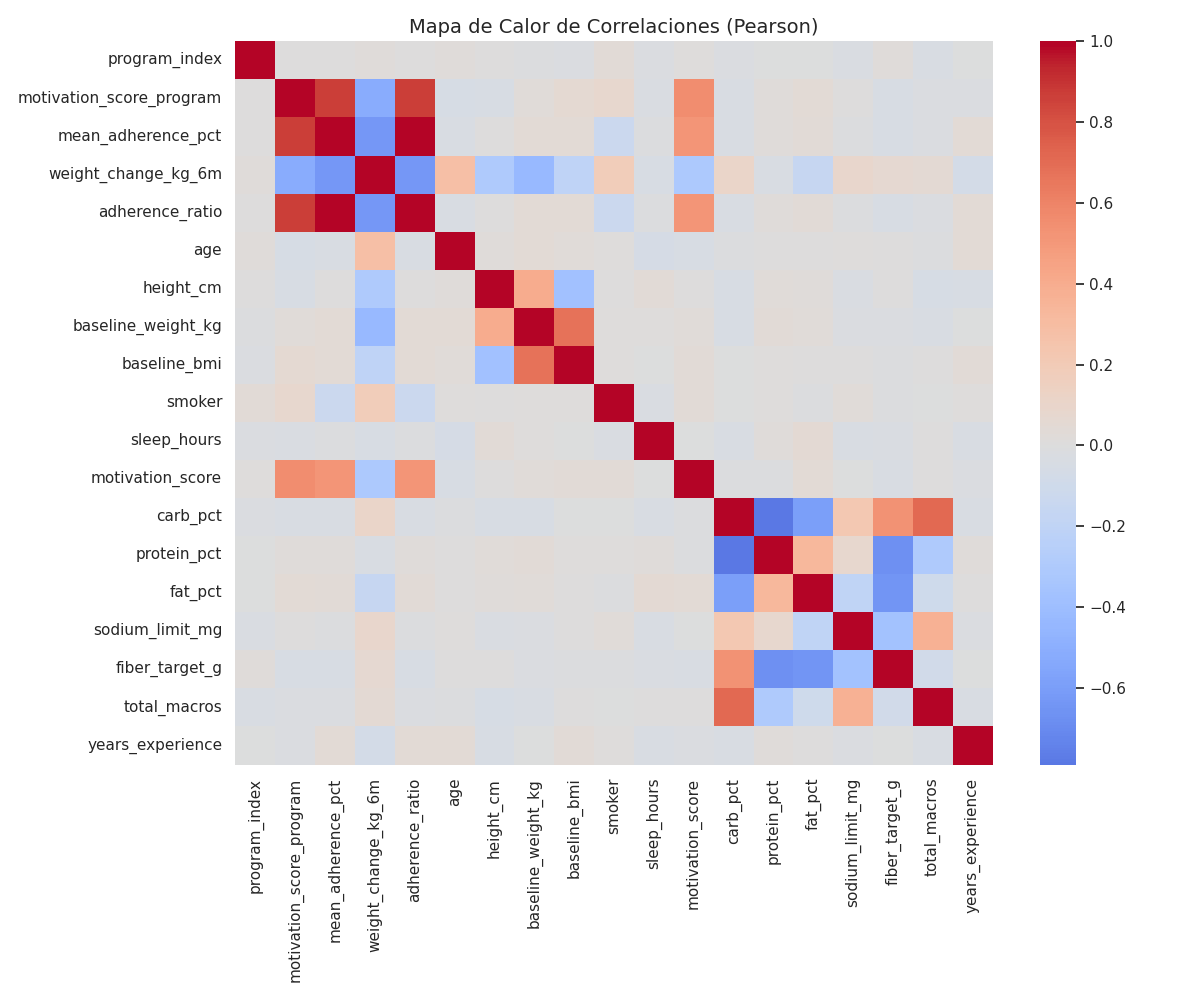
\includegraphics[width=0.9\textwidth]{heatmap_correlacion.png}
\caption{Mapa de calor das correlações de Pearson entre as variáveis numéricas.}
\label{fig:heatmap}
\end{figure}

\section{Resultados por Tipo de Dieta}
A análise da perda média de peso por tipo de dieta mostrou diferenças, embora moderadas. As dietas de baixo teor de hidratos de carbono, agrupadas em \texttt{Low\_carb}, apresentam a maior perda média, próxima de 24 kg. Seguem-se as dietas de base vegetal e as ricas em proteína, e por fim as equilibradas, com perda média de cerca de 21 kg. A diferença entre o melhor e o pior tipo de dieta é de aproximadamente 3 kg em média, o que sugere que o tipo de dieta tem influência, mas não é o fator dominante. A figura \ref{fig:dietas} mostra a distribuição da variação de peso para cada tipo de dieta.

\begin{figure}[h]
\centering
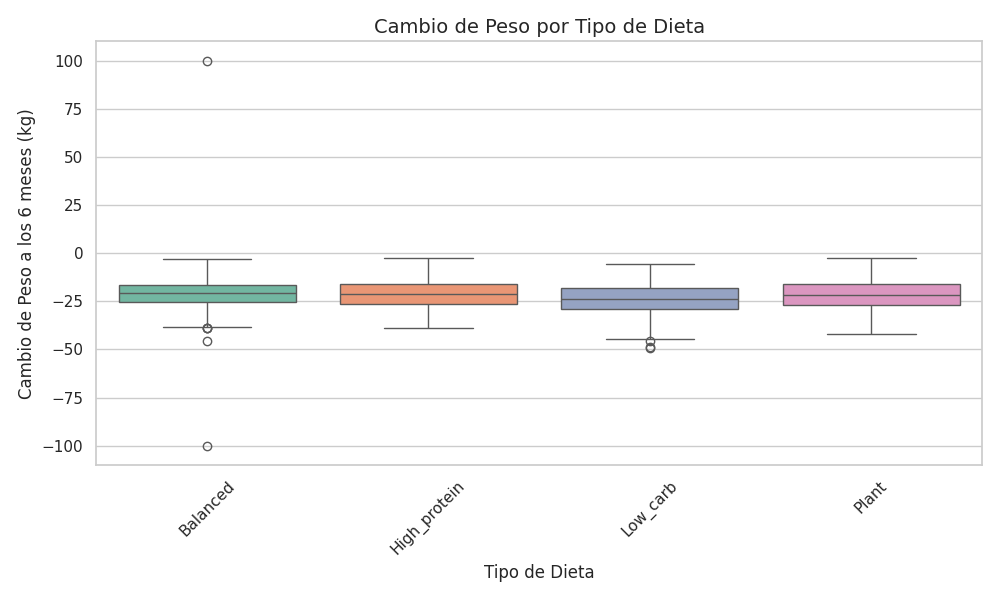
\includegraphics[width=0.8\textwidth]{boxplot_dietas.png}
\caption{Variação de peso aos seis meses por tipo de dieta.}
\label{fig:dietas}
\end{figure}

\section{Resultados por Sexo}
A comparação por sexo revelou uma diferença assinalável. Os pacientes do sexo masculino apresentam uma perda média de cerca de 24,9 kg, enquanto as pacientes do sexo feminino apresentam uma perda média de cerca de 19,3 kg. A diferença média entre os dois grupos é de aproximadamente 5,6 kg.

Esta diferença é relevante, mas deve ser interpretada com cuidado. Parte dela pode dever-se a fatores fisiológicos, já que a perda de peso depende da composição corporal, mas pode também refletir diferenças noutras variáveis distribuídas de forma desigual entre os dois grupos. A figura \ref{fig:sexo} apresenta a distribuição da variação de peso para cada sexo.

\begin{figure}[h]
\centering
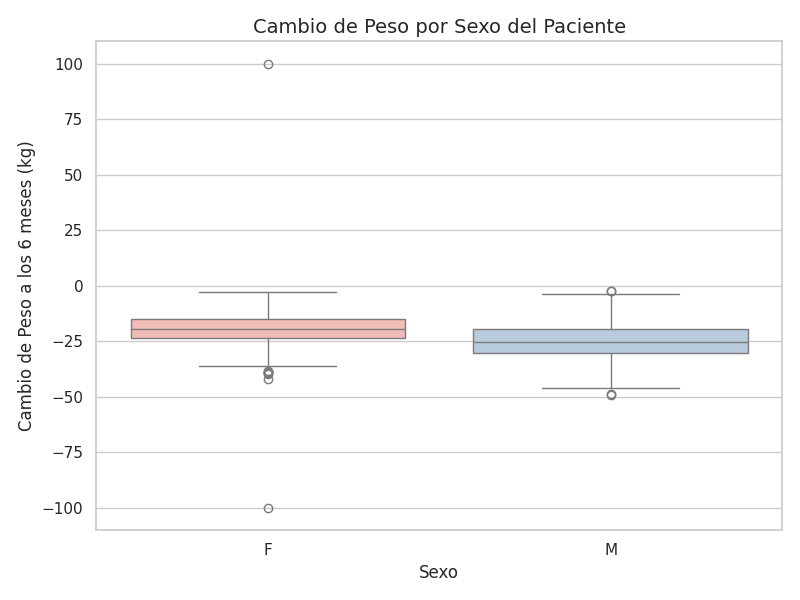
\includegraphics[width=0.65\textwidth]{boxplot_sexo.png}
\caption{Variação de peso aos seis meses por sexo do paciente.}
\label{fig:sexo}
\end{figure}

Importa ainda referir que foi precisamente esta análise por sexo que tornou visível o problema de inconsistência na coluna \texttt{sex}, descrito no capítulo anterior. Numa execução inicial, o resumo apresentou oito grupos em vez de dois, o que levou o grupo a reforçar a normalização desta coluna.

\section{Influência do Perfil do Nutricionista}
O grupo analisou o efeito da abordagem do nutricionista no resultado das dietas. Os resultados mostram que a abordagem mais exigente, identificada como \texttt{Strict}, está associada à maior perda média de peso, cerca de 23,8 kg. As abordagens \texttt{Motivational} e \texttt{Empathetic} situam-se em valores intermédios, e a abordagem \texttt{Data\_driven} apresenta a menor perda média, cerca de 20,4 kg. Já a especialidade do nutricionista mostrou pouca influência, com perdas médias muito próximas entre as quatro especialidades, todas entre 21,7 e 22,1 kg. A figura \ref{fig:nutricionista} apresenta a perda média de peso para cada abordagem.

\begin{figure}[h]
\centering
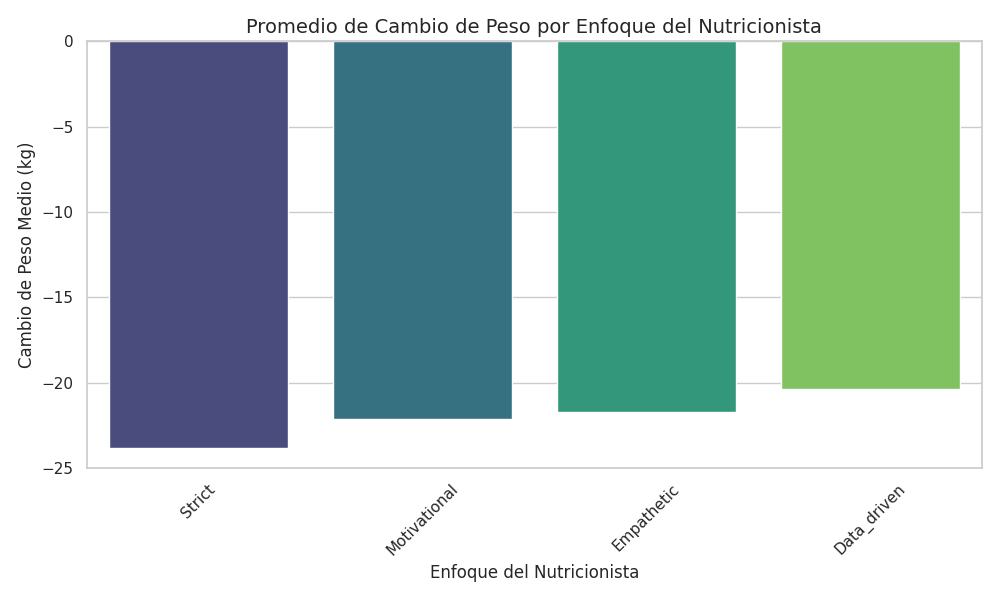
\includegraphics[width=0.8\textwidth]{barras_nutricionista.png}
\caption{Perda média de peso por abordagem do nutricionista.}
\label{fig:nutricionista}
\end{figure}

\section{Síntese da Análise}
Desta fase ficaram duas conclusões principais. A primeira é que o comportamento do paciente, traduzido na adesão e na motivação, é de longe o fator mais ligado ao resultado, mais do que qualquer característica da dieta ou do nutricionista. A segunda é que existem variáveis redundantes no conjunto, nomeadamente o par formado pela adesão e pelo rácio de adesão, que devem ser tratadas com cuidado na modelação.

\chapter{Identificação de Padrões e Modelos de Previsão}
\label{chap:modelos}

\section{Identificação de Padrões por Clustering}
A análise exploratória do capítulo anterior revelou relações diretas entre pares de variáveis. Para procurar padrões mais complexos, que envolvam várias variáveis ao mesmo tempo, o grupo recorreu a aprendizagem não supervisionada. Esta parte foi implementada no \textit{script} \texttt{clustering.py}.

\subsection{Método Utilizado}
O algoritmo escolhido foi o \textit{K-Means}~\cite{geron}, por ser simples de interpretar e adequado a variáveis numéricas. Foram usadas como entrada cinco características relevantes para descrever o perfil dos pacientes e o seu resultado: idade, peso inicial, motivação, adesão média e variação de peso aos seis meses.

Antes da aplicação do algoritmo, todas as variáveis foram padronizadas com o \textit{StandardScaler}. Este passo é necessário porque o \textit{K-Means} se baseia em distâncias, e sem padronização as variáveis de maior escala, como o peso, dominariam o cálculo face a variáveis de menor escala, como a motivação. O número de grupos foi fixado em quatro, com o objetivo de identificar quatro perfis distintos de pacientes.

\subsection{Perfis Encontrados}
A tabela \ref{tab:clusters} resume os quatro grupos identificados.

\begin{table}[h]
\centering
\begin{tabular}{|c|r|c|c|c|c|}
\hline
\textbf{Grupo} & \textbf{Pacientes} & \textbf{Idade} & \textbf{Motivação} & \textbf{Adesão} & \textbf{Perda de peso} \\
\hline
0 & 842 & 31,3 & 0,78 & 85,7\% & $-27,8$ kg \\
1 & 744 & 56,9 & 0,79 & 85,5\% & $-22,2$ kg \\
2 & 642 & 44,9 & 0,55 & 59,9\% & $-13,9$ kg \\
3 & 5 & 42,0 & 5,00 & 79,2\% & $-23,8$ kg \\
\hline
\end{tabular}
\caption{Perfil médio de cada grupo identificado por \textit{clustering}.}
\label{tab:clusters}
\end{table}

A leitura dos três grupos principais conta uma história clara. O grupo 0 reúne os pacientes mais jovens, com idade média de 31 anos, alta adesão e a maior perda de peso. O grupo 1 reúne pacientes mais velhos, com idade média de 57 anos, com a mesma motivação e adesão dos mais jovens, mas com menor perda de peso. Esta diferença entre os grupos 0 e 1, com comportamento semelhante mas resultados diferentes, é coerente com o efeito da idade no metabolismo. O grupo 2 reúne os pacientes com motivação e adesão mais baixas, e é, como seria de esperar, o que perde menos peso.

A figura \ref{fig:clusters} mostra a distribuição dos pacientes segundo o peso inicial e a variação de peso, com cada grupo representado por uma cor. O gráfico permite ainda observar a presença de dois pontos isolados, com variações de peso próximas de mais e menos 100 kg, que correspondem a valores extremos não tratados pelo \textit{capping}, uma vez que este foi aplicado apenas às variáveis de idade, peso e altura.

\begin{figure}[h]
\centering
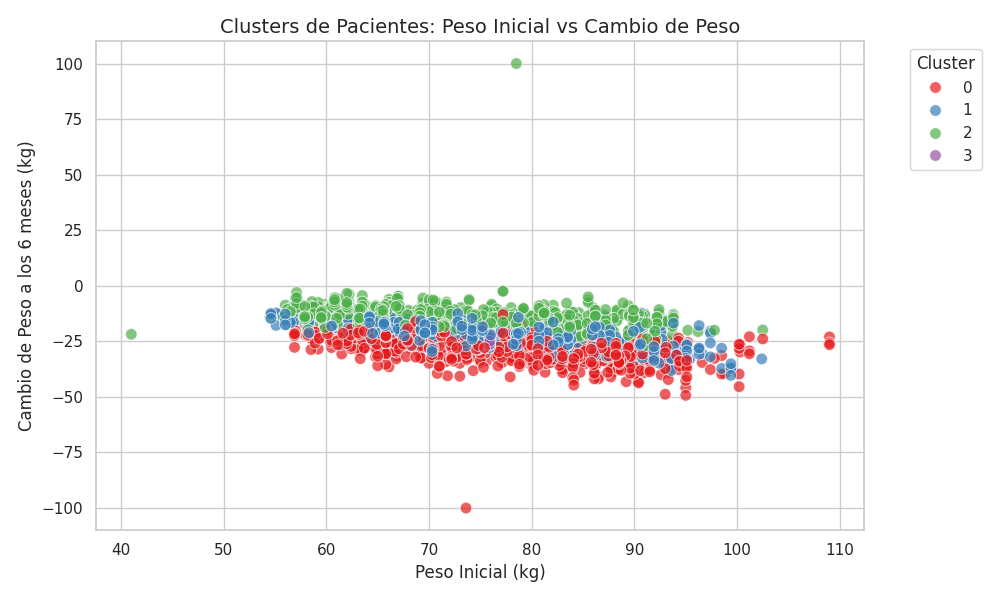
\includegraphics[width=0.85\textwidth]{clusters_peso.png}
\caption{Grupos de pacientes segundo o peso inicial e a variação de peso.}
\label{fig:clusters}
\end{figure}

\subsection{O Grupo Anómalo e a Qualidade dos Dados}
O grupo 3 merece destaque próprio. Contém apenas cinco registos e distingue-se por um valor de motivação de exatamente 5,0, enquanto todos os outros pacientes apresentam valores entre 0,15 e 0,99. Este valor não corresponde a pacientes extraordinariamente motivados, mas a um erro na introdução dos dados. Estes registos foram provavelmente preenchidos numa escala de 1 a 5, em vez da escala de 0 a 1 usada no resto do conjunto.

O facto de o \textit{K-Means} ter isolado automaticamente estes cinco registos num grupo próprio é, em si, um resultado relevante. Mostra que as técnicas de \textit{clustering}, para além de identificarem perfis de pacientes, funcionam também como uma ferramenta de deteção de problemas de qualidade dos dados que tinham passado despercebidos nas fases anteriores. Este foi um achado útil que o grupo registou para discussão.

\section{Aplicação de Modelos de Previsão}
A última fase de análise consistiu na aplicação de modelos de aprendizagem supervisionada, implementados no \textit{script} \texttt{predictive\_modeling.py} com recurso à biblioteca \textit{scikit-learn}~\cite{scikit}. O objetivo foi prever a variável \texttt{weight\_change\_kg\_6m}, ou seja, a quantidade de peso perdido ao fim de seis meses, tratando o problema como uma regressão.

\subsection{Seleção de Variáveis e Prevenção de Data Leakage}
A seleção das variáveis preditoras foi a decisão mais importante desta fase. Em primeiro lugar, foram removidas as colunas de identificação, como os identificadores de paciente, dieta e nutricionista, por não terem qualquer valor preditivo.

Em segundo lugar, e mais importante, foram removidas as variáveis que só são conhecidas durante ou depois do programa de dieta, nomeadamente a adesão média, o rácio de adesão, a motivação registada durante o programa e o índice do programa. A razão para esta remoção é evitar um problema conhecido como \textit{data leakage}. Se o modelo usasse a adesão para prever a perda de peso, estaria a usar informação que, na prática, ainda não existe no momento em que a previsão é útil, isto é, antes de a dieta começar. Um modelo treinado com essa informação teria um desempenho aparentemente excelente, mas seria inútil numa situação real. Ao remover estas variáveis, o grupo garantiu que o modelo só usa informação disponível à partida: características do paciente, da dieta e do nutricionista.

As variáveis categóricas restantes foram transformadas em variáveis numéricas através de codificação \textit{one-hot}. O conjunto final de características ficou com 33 colunas.

\subsection{Treino e Avaliação}
Os dados foram divididos em conjunto de treino, com 80\% das linhas, e conjunto de teste, com os restantes 20\%. Foram treinados três modelos de naturezas diferentes: uma regressão linear, uma \textit{random forest} e um \textit{gradient boosting}. A tabela \ref{tab:reg} apresenta os resultados no conjunto de teste, medidos pelo erro quadrático médio, pela sua raiz e pelo coeficiente de determinação.

\begin{table}[h]
\centering
\begin{tabular}{|l|c|c|c|}
\hline
\textbf{Modelo} & \textbf{MSE} & \textbf{RMSE (kg)} & \textbf{$R^2$} \\
\hline
Regressão linear & 18,54 & 4,31 & 0,655 \\
\textit{Random forest} & 10,98 & 3,31 & 0,796 \\
\textit{Gradient boosting} & 11,69 & 3,42 & 0,783 \\
\hline
\end{tabular}
\caption{Desempenho dos modelos de regressão no conjunto de teste.}
\label{tab:reg}
\end{table}

Os modelos baseados em árvores, a \textit{random forest} e o \textit{gradient boosting}, tiveram um desempenho claramente superior ao da regressão linear. A \textit{random forest} foi o melhor modelo, com um coeficiente de determinação de 0,796 e um erro médio de cerca de 3,3 kg. A análise destes resultados é aprofundada no capítulo seguinte.

\chapter{Discussão Crítica e Conclusões}
\label{chap:conclusoes}

\section{Comparação dos Modelos}
Os resultados da fase de modelação mostram uma diferença clara entre a regressão linear e os modelos baseados em árvores. A regressão linear obteve o pior desempenho, com um coeficiente de determinação de 0,655. A \textit{random forest} e o \textit{gradient boosting} ficaram bastante acima, com valores de 0,796 e 0,783 respetivamente.

A razão para o desempenho mais fraco da regressão linear está na sua própria natureza. Este modelo assume que a relação entre as variáveis e o resultado é linear, ou seja, que cada variável contribui de forma fixa e independente das outras. A perda de peso, porém, é um processo biológico complexo, em que fatores como a idade, o peso inicial e o tipo de dieta interagem entre si de formas não lineares. O efeito de uma dieta não é o mesmo num paciente jovem e num paciente mais velho, e a regressão linear não consegue captar esse tipo de interação.

Os modelos baseados em árvores não têm essa limitação. Ao dividirem os dados sucessivamente segundo as várias variáveis, conseguem representar interações e relações não lineares de forma natural. O \textit{gradient boosting} e a \textit{random forest} combinam ainda muitas árvores, o que reduz o sobreajuste que afetaria uma árvore isolada. É essa capacidade de captar padrões complexos que explica o seu melhor desempenho.

Entre os dois modelos de conjunto, a \textit{random forest} obteve neste trabalho um resultado ligeiramente superior ao do \textit{gradient boosting}. Os dois modelos são, ainda assim, de qualidade próxima, e ambos seriam escolhas defensáveis. O grupo considera a \textit{random forest} como o melhor modelo deste estudo, por ter apresentado o maior coeficiente de determinação e o menor erro no conjunto de teste.

\section{Interpretação dos Resultados}
A conclusão mais sólida de todo o trabalho é que o resultado de uma dieta depende sobretudo do comportamento do paciente. A adesão ao plano e a motivação foram, em todas as fases da análise, os fatores mais ligados à perda de peso. Em termos práticos, isto sugere que, para um profissional de saúde, garantir que o paciente segue o plano é mais determinante do que a escolha entre uma dieta e outra.

O tipo de dieta tem influência, mas pequena. A diferença de perda média entre o melhor e o pior tipo de dieta foi de cerca de 3 kg. O perfil do nutricionista mostrou um efeito moderado, com a abordagem mais exigente associada a melhores resultados, enquanto a especialidade se mostrou praticamente irrelevante.

Importa sublinhar que o melhor modelo consegue prever a perda de peso com um erro médio na ordem dos 3,3 kg, usando apenas informação conhecida antes do início da dieta. Este resultado mostra que existe valor preditivo real nas características do paciente, da dieta e do nutricionista, mesmo sem recorrer a dados de adesão.

\section{Limitações do Trabalho}
O grupo identificou várias limitações que condicionam a leitura dos resultados. A primeira diz respeito à variável de resultado. No conjunto de dados, todos os programas registaram perda de peso, sem um único caso de ganho ou de manutenção. Um conjunto de dados realista de acompanhamento nutricional teria também casos de insucesso. Esta ausência faz com que o problema não distinga propriamente sucesso de fracasso, mas sim graus de sucesso.

A segunda limitação está na divisão dos dados. O \textit{script} de modelação usa uma divisão de 80\% para treino e 20\% para teste. O enunciado sugeria uma divisão diferente, com conjuntos de treino, validação e teste, e uma parte reservada não utilizada. Numa versão futura, ajustar a divisão a esse esquema permitiria uma otimização de hiperparâmetros mais rigorosa e uma avaliação mais robusta.

A terceira limitação é que o trabalho se centrou na previsão da quantidade de peso perdido, tratada como regressão. Uma extensão natural seria abordar também o problema como classificação, definindo uma variável binária de sucesso e prevendo diretamente a probabilidade de uma dieta resultar.

Por fim, a deteção dos cinco registos anómalos no \textit{clustering}, com motivação fora de escala, mostra que ainda podem existir outros erros de qualidade não detetados no conjunto de dados.

\section{Trabalho Futuro}
A partir das limitações identificadas, o grupo aponta algumas direções de melhoria. A primeira seria trabalhar com um conjunto de dados que incluísse casos de insucesso reais, tornando os modelos capazes de distinguir bons e maus resultados. A segunda seria implementar o esquema de divisão de dados sugerido no enunciado e usar essa estrutura para otimizar os hiperparâmetros dos modelos. A terceira seria acrescentar um modelo de classificação do sucesso da dieta, complementando a abordagem de regressão já desenvolvida.

\section{Conclusão}
O trabalho percorreu todas as etapas de um processo de análise de dados, da integração dos quatro ficheiros até à aplicação e discussão de modelos de previsão. As principais conclusões são que o comportamento do paciente, sobretudo a adesão ao plano, é o fator mais determinante para o resultado de uma dieta, e que é possível prever a perda de peso com um erro médio de cerca de 3,3 kg usando apenas informação disponível à partida. O processo permitiu ainda detetar, através do \textit{clustering}, problemas de qualidade nos dados que não eram visíveis de outra forma. As limitações identificadas mostram que estas conclusões devem ser entendidas no contexto do conjunto de dados fornecido, mas a metodologia desenvolvida é aplicável a dados mais completos.


% bibliografia
\bibliographystyle{plain}
\bibliography{bibliografia}

\end{document}
